\chapter{Feature Scoring and Selection}
\label{ch:reg-fss}

Linear regression infers a model that estimates the class, a real-valued feature, as a sum of products of input features and their weights. Consider the data on prices of imported cars in 1985. Inspecting this data set in a \widget{Data Table} shows that some features, like fuel-system, engine-type, and many others, are discrete. Linear regression only works with numbers. In Orange, linear regression will automatically convert all discrete values to numbers, often using several features to represent a single discrete feature. We also do this conversion manually by using the \widget{Continuize} widget.

\begin{figure}[h]
    \centering
    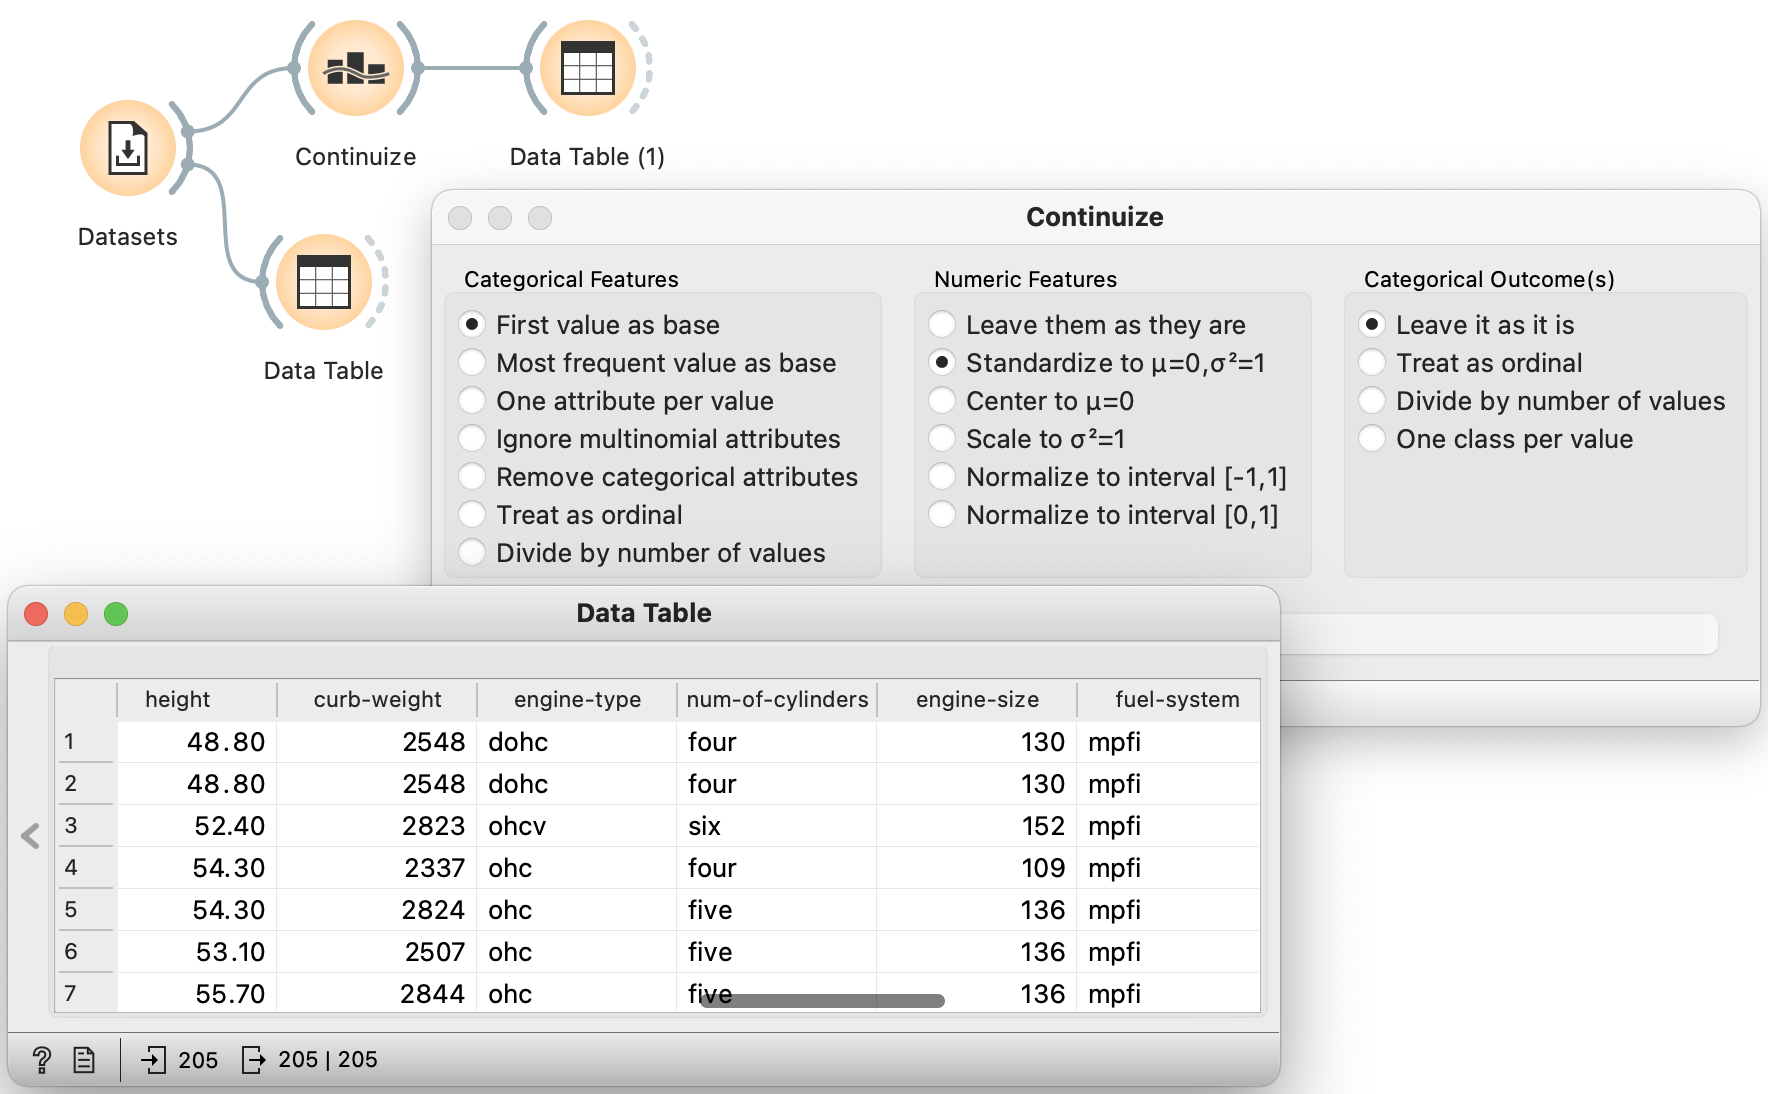
\includegraphics[scale=0.5]{workflow-continuize.png}
    \caption{$\;$}
\end{figure}

Before continuing, you should check what \widget{Continuize} does and how it converts the nominal features into real-valued features. The table below should provide sufficient illustration.

\begin{figure}[h]
    \centering
    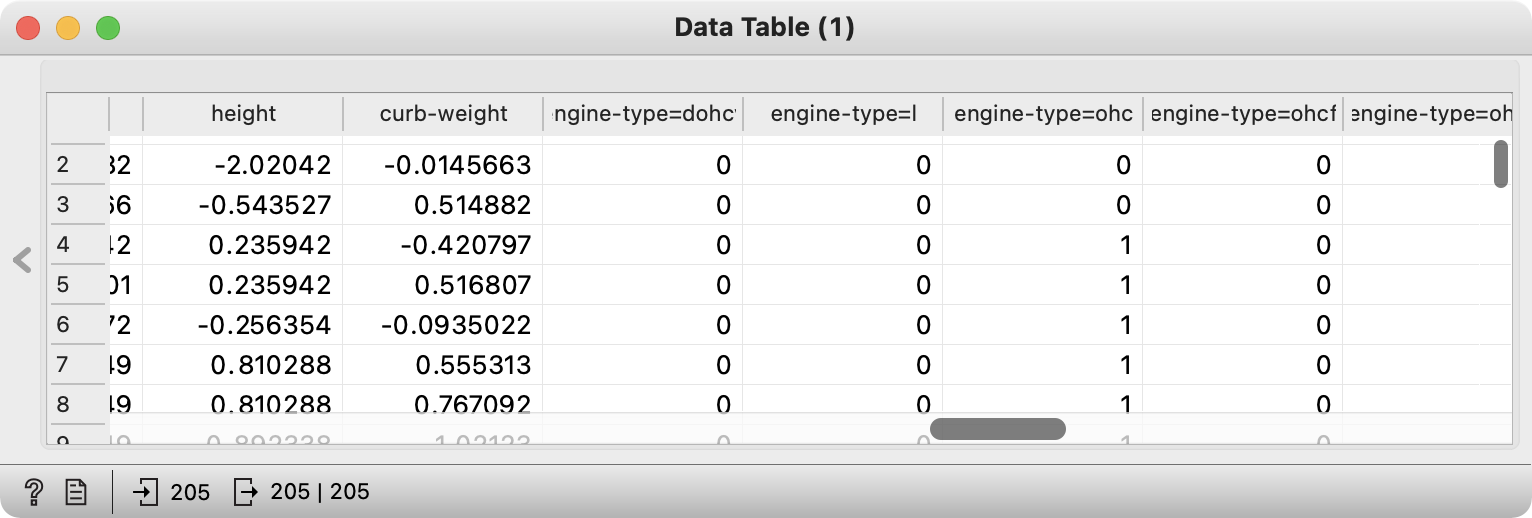
\includegraphics[scale=0.5]{after-continuize.png}
    \caption{$\;$}
\end{figure}

Now to the core of this lesson. Our workflow reads the data continuizes it such that we also normalize all the features to bring them to equal scale. We then load the data into the {\em Linear Regression} widget and check out the feature coefficients in the \widget{Data Table}.

\begin{figure}[h]
    \centering
    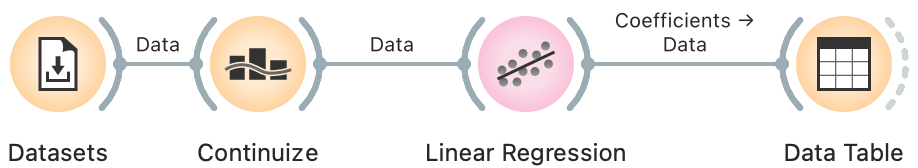
\includegraphics[scale=0.5]{workflow-cont-lr.png}
    \caption{$\;$}
\end{figure}

In \widget{Linear Regression}, we will use L1 regularization. Compared to L2 regularization, which aims to minimize the sum of squared weights, L1 regularization is rougher: it minimizes the sum of absolute values of the weights. The result of this ``roughness'' is that many of the features will get zero weights. But this feature elimination may also be exactly what we want. We want to select only the most important features and see how the model that uses only a smaller subset of features behaves. Also, this smaller set of features is ranked. Engine size is a huge factor in the pricing of our cars, and so is the make, where Porsche, Mercedes, and BMW cost more than other cars (ok, no news here).

\begin{figure}[h]
    \centering
    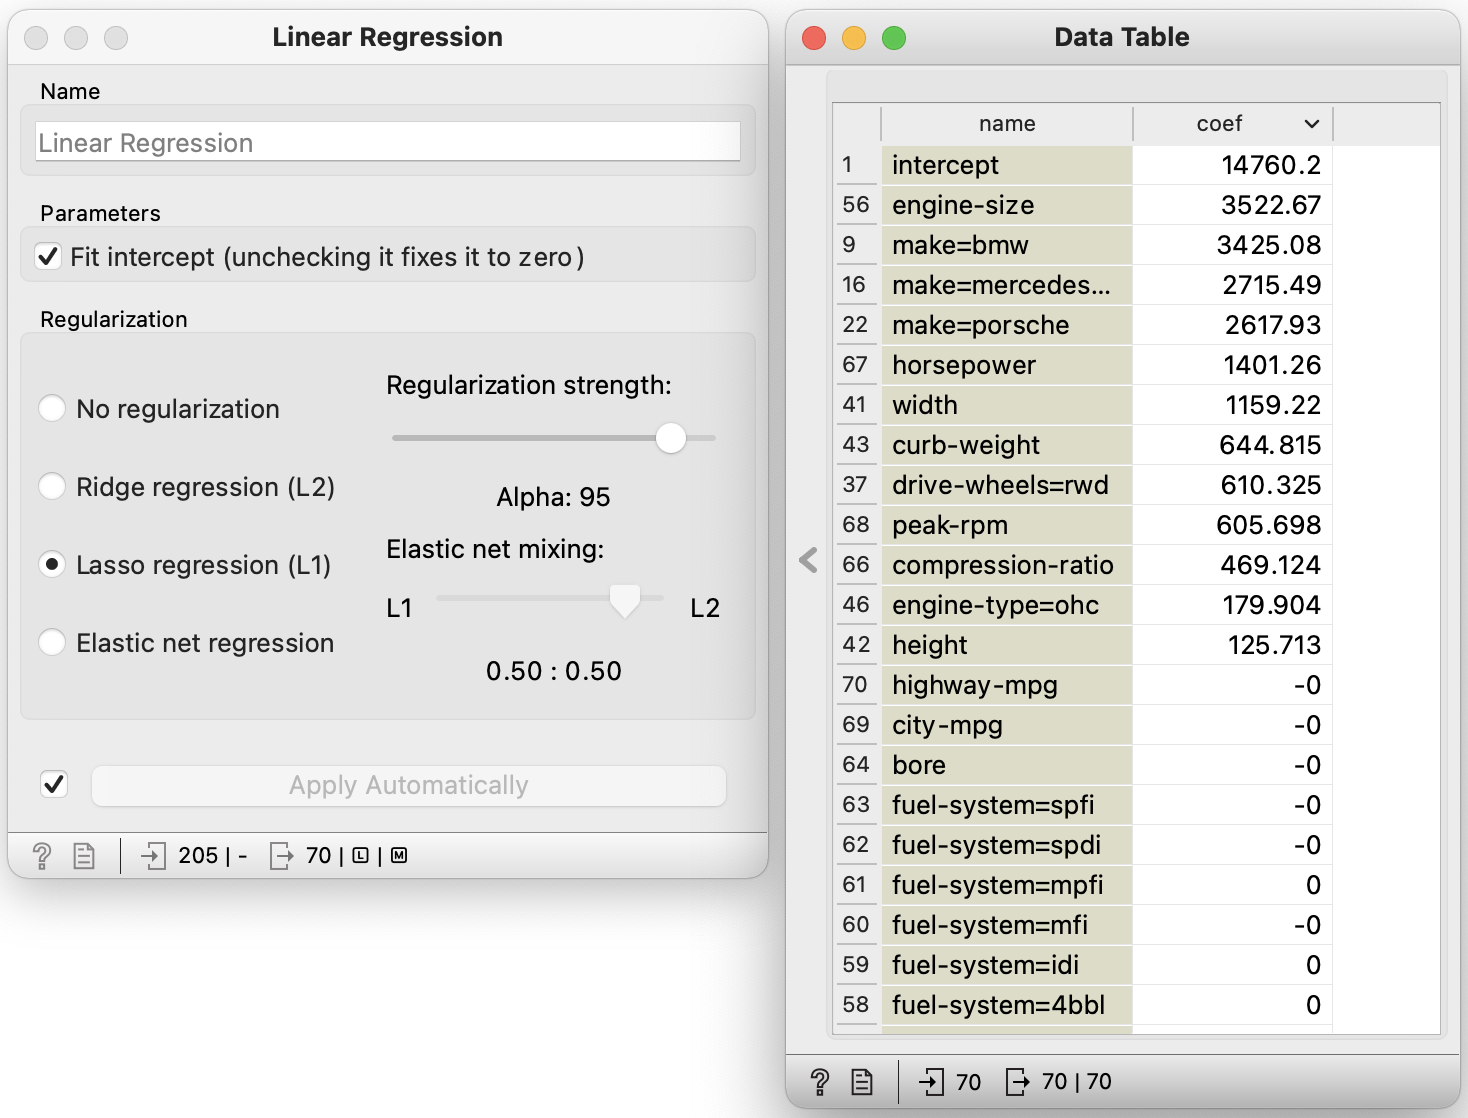
\includegraphics[scale=0.4]{coefficients.png}
    \caption{$\;$}
\end{figure}

We should\marginnote{\textbf{\textsf{We care about features with substantial weights, regardless of their sign. Therefore, we should change the workflow to compute and show the data features by their absolute weight. Could you change the workflow accordingly? Hint: use the Feature Construction widget.}}} notice that the number of features with non-zero weights varies with regularization strength. Stronger regularization would result in fewer features with non-zero weights.

